\section{Mathematische Logik}
\label{sec:fundamentals_mathematical_logic}

Mathematische Aussagen bilden die Grundlage für Definitionen, Sätze und
Beweise. Entscheidend ist dabei nicht nur, ob eine Aussage wahr oder unwahr ist,
sondern ob sich dies auch eindeutig und objektiv feststellen lässt.

\begin{DefinitionBox}{Aussage}{fundamentals_mathematical_statement}
  Eine \emph{Aussage} \EnglishTerm{statement} ist ein sprachlicher oder
  mathematischer Ausdruck, dem eindeutig einer der beiden Wahrheitswerte
  \emph{wahr}, abgekürzt T \EnglishTerm{true}, oder \emph{falsch}, abgekürzt F
  \EnglishTerm{false}, zugeordnet werden kann.
\end{DefinitionBox}

\begin{ExampleBox}{Aussagen und Wahrheitswerte}{fundamentals_statement_examples}
  \begin{enumerate}[label=(\alph*),itemsep=0.4em]
    \item \emph{„Die Zahl $11$ ist eine Primzahl.“} \\
    Das ist \Cloze{3cm}{eine valide} Aussage im mathematischen Sinne. Sie ist \Cloze{2.5cm}{wahr (T)}.
    \item \emph{„Die Zahl 3 ist kleiner als die Zahl 2.“} oder
    \emph{„$3<2$“} \\
    Das ist \Cloze{3cm}{eine valide} Aussage im mathematischen Sinne. Sie ist \Cloze{2.5cm}{falsch (F)}.
    \item \emph{„Ich spreche jetzt nicht die Wahrheit.“}
    (Russell-Paradoxon, 1903) \\
    Das ist \Cloze{3cm}{keine} Aussage im mathematischen Sinne, da sie nicht widerspruchsfrei als wahr oder falsch bewertet werden kann.
  \end{enumerate}
\end{ExampleBox}



\subsection{Logische Verknüpfungen}
\label{subsec:fundamentals_logical_connectives}

Durch die Verknüpfung zweier Aussagen $A$ und $B$ lassen sich neue Aussagen bilden:

\begin{DefinitionBox}{UND-Verknüpfung}{fundamentals_and_connective}
  Die \emph{UND-Verknüpfung}, fachsprachlich \emph{Konjunktion}
  \EnglishTerm{conjunction},
  \[
    A\land B,
  \]
  ist nur dann wahr, wenn sowohl $A$ als auch $B$ wahr sind. Ist mindestens eine
  der beiden Aussagen falsch, so ist auch $A\land B$ falsch.
\end{DefinitionBox}

\begin{DefinitionBox}{ODER-Verknüpfung}{fundamentals_or_connective}
  Die \emph{ODER-Verknüpfung}, fachsprachlich \emph{Disjunktion}
  \EnglishTerm{disjunction},
  \[
    A\lor B,
  \]
  ist wahr, wenn mindestens eine der beiden Aussagen $A$ und $B$ wahr ist. Sie
  ist nur dann falsch, wenn beide Aussagen falsch sind.
\end{DefinitionBox}

\begin{samepage}
Eine Wahrheitstabelle erfasst alle möglichen Wahrheitswerte von $A$ und $B$;
durch das Ausfüllen erkennen wir systematisch, wann die UND- und die
ODER-Verknüpfung wahr oder falsch sind.

\begin{center}
  \renewcommand{\arraystretch}{1.55}
  \setlength{\tabcolsep}{12pt}
  \begin{tabular}{cccc}
    \toprule
    $A$ & $B$ & $A\land B$ & $A\lor B$\\
    \midrule
    T & T & \Cloze{1.8cm}{T} & \Cloze{1.8cm}{T}\\
    T & F & \Cloze{1.8cm}{F} & \Cloze{1.8cm}{T}\\
    F & T & \Cloze{1.8cm}{F} & \Cloze{1.8cm}{T}\\
    F & F & \Cloze{1.8cm}{F} & \Cloze{1.8cm}{F}\\
    \bottomrule
  \end{tabular}
\end{center}
\end{samepage}

\begin{RemarkBox}
  Das mathematische ODER ist grundsätzlich inklusiv, d.\,h. $A\lor B$ ist auch
  dann wahr, wenn sowohl $A$ als auch $B$ wahr sind. Im Gegensatz dazu gibt es
  in der Informatik auch das exklusive Oder, das nur dann wahr ist, wenn genau
  eine (aber nicht beide) der Aussagen wahr ist.
\end{RemarkBox}

\subsection{Implikation und Äquivalenz}
\label{subsec:fundamentals_implication_and_equivalence}

Mit Implikationen und Äquivalenzen stellen wir logische Zusammenhänge zwischen
Aussagen her und können präzise beschreiben, wie die Gültigkeit einer Aussage
von einer anderen abhängt.

\begin{DefinitionBox}{Implikation}{fundamentals_implication}
  Die \emph{Implikation} \EnglishTerm{implication} zeigt an, welche Aussage aus einer anderen folgt:
  \[
    A\Rightarrow B
  \]
  bedeutet: „Wenn $A$ gilt, dann gilt auch $B$.“
\end{DefinitionBox}


\begin{RemarkBox}
  Eine Implikation gilt nicht notwendigerweise in beide Richtungen: Aus
  $A\Rightarrow B$ folgt im Allgemeinen nicht $B\Rightarrow A$.
\end{RemarkBox}

\begin{ExampleBox}{Implikation}{fundamentals_implication_example}
  Für eine ganze Zahl $x$ gilt die folgende Implikation:
  \[
    x=4
    \quad\Rightarrow\quad
    x \text{ ist gerade}.
  \]
  Dreht man den Implikationspfeil lediglich um, erhält man dagegen eine falsche
  Aussage:
    \begin{center}
      \begin{ClozeArea}[0.6\linewidth]{1.5cm}
      \[
           x \text{ ist gerade} \quad \nRightarrow \quad x=4.
      \]
      \end{ClozeArea}
    \end{center}
  Das Gegenbeispiel $x=2$ widerlegt die Aussage.
\end{ExampleBox}

\begin{DefinitionBox}{Äquivalenz}{fundamentals_equivalence}
  Die \emph{Äquivalenz} \EnglishTerm{equivalence}
  \[
    A\Leftrightarrow B
  \]
  bedeutet, dass sowohl $A\Rightarrow B$ als auch $B\Rightarrow A$ gilt. Das bedeutet, dass die Aussagen $A$ und $B$ äquivalent, also logisch gleichwertig sind. Sie sind entweder beide wahr oder beide falsch.
\end{DefinitionBox}

\begin{samepage}
Eine Wahrheitstabelle prüft alle möglichen Fälle; durch das Ausfüllen sehen wir,
unter welchen Wahrheitswerten eine Implikation oder eine Äquivalenz gilt.

\begin{center}
  \renewcommand{\arraystretch}{1.55}
  \setlength{\tabcolsep}{12pt}
  \begin{tabular}{cccc}
    \toprule
    $A$ & $B$ & $A\Rightarrow B$ & $A\Leftrightarrow B$\\
    \midrule
    T & T & \Cloze{1.8cm}{T} & \Cloze{1.8cm}{T}\\
    T & F & \Cloze{1.8cm}{F} & \Cloze{1.8cm}{F}\\
    F & T & \Cloze{1.8cm}{T} & \Cloze{1.8cm}{F}\\
    F & F & \Cloze{1.8cm}{T} & \Cloze{1.8cm}{T}\\
    \bottomrule
  \end{tabular}
\end{center}
\end{samepage}

Bei einer Implikation ist $A$ eine hinreichende Bedingung für $B$ und $B$ eine
notwendige Bedingung für $A$. Für eine Äquivalenz müssen diese Beziehungen in
beiden Richtungen gelten.

\subsection{Negation}
\label{subsec:fundamentals_negation}

Negationen sind wesentlich, weil wir mit ihnen das Gegenteil einer Aussage
präzise ausdrücken und dadurch logische Zusammenhänge systematisch untersuchen
können.

\begin{DefinitionBox}{Negation}{fundamentals_negation}
  Die \emph{Negation} \EnglishTerm{negation} einer Aussage $A$ wird mit
  $\neg A$ bezeichnet und kehrt den Wahrheitswert von $A$ um: Ist $A$ wahr, so
  ist $\neg A$ falsch; ist $A$ falsch, so ist $\neg A$ wahr.
\end{DefinitionBox}

\begin{ExampleBox}{Negation von Aussagen}{fundamentals_negation_example}
  Negieren Sie jeweils die angegebene Aussage $A$.
  \begin{enumerate}[label=(\alph*),itemsep=0.8em]
    \item Für eine feste reelle Zahl $x$:
      \par\smallskip
      \makebox[1.5cm][l]{$A:$}$x>5$\\[0.4em]
      \makebox[1.5cm][l]{$\neg A:$}\Cloze{5cm}{$x\leq 5$}

    \item
      \par\smallskip
      \makebox[1.5cm][l]{$A:$}„Die Zahl $17$ ist eine Primzahl.“\\[0.4em]
      \makebox[1.5cm][l]{$\neg A:$}\Cloze{9cm}{„Die Zahl $17$ ist keine Primzahl.“}

    \item
      \par\smallskip
      \makebox[1.5cm][l]{$A:$}„Heute regnet es.“\\[0.4em]
      \makebox[1.5cm][l]{$\neg A:$}\Cloze{9cm}{„Heute regnet es nicht.“}
  \end{enumerate}
\end{ExampleBox}

Wendet man eine Negation auf eine UND- oder ODER-Verknüpfung an, so muss man die
de-morganschen Regeln berücksichtigen. Mit dem zuvor eingeführten
Äquivalenzzeichen lassen sich diese präzise formulieren.

\begin{TheoremBox}{De-morgansche Regeln}{fundamentals_de_morgan_rules}
  Beim Negieren einer Verknüpfung werden UND und ODER miteinander vertauscht
  und beide Teilaussagen negiert:
  \[
    \neg(A\land B)\Leftrightarrow (\neg A)\lor(\neg B),
  \]
  \[
    \neg(A\lor B)\Leftrightarrow (\neg A)\land(\neg B).
  \]
\end{TheoremBox}

\begin{ExampleBox}{De-morgansche Regeln}{fundamentals_de_morgan_rules_example}
  Es seien $a,b,x\in\R$ mit $a\leq b$. Nach der zweiten de-morganschen Regel
  gilt
  \begin{align*}
    \neg\bigl((x<a)\lor(x>b)\bigr)
      &\Leftrightarrow
        \Cloze{7.2cm}{\neg(x<a)\land\neg(x>b)}\\
      &\Leftrightarrow
        \Cloze{7.2cm}{(x\geq a)\land(x\leq b)}.
  \end{align*}

  \begin{center}
    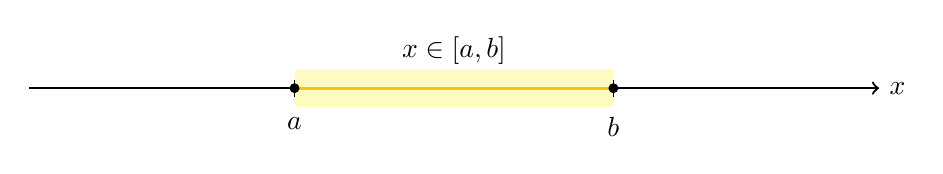
\begin{tikzpicture}[x=1.35cm,y=1cm]
  \fill[yellow!70,opacity=0.35] (-1.5,-0.24) rectangle (1.5,0.24);
  \draw[->,thick] (-4,0) -- (4,0) node[right] {$x$};
  \draw[very thick,yellow!55!orange] (-1.5,0) -- (1.5,0);
  \fill (-1.5,0) circle (1.8pt);
  \fill (1.5,0) circle (1.8pt);
  \draw (-1.5,0.11) -- (-1.5,-0.11) node[below=4pt] {$a$};
  \draw (1.5,0.11) -- (1.5,-0.11) node[below=4pt] {$b$};
  \node[above=5pt] at (0,0) {$x\in[a,b]$};
\end{tikzpicture}

  \end{center}

  Die ursprüngliche Aussage schließt aus, dass $x$ links von $a$ oder rechts
  von $b$ liegt. Daher muss gleichzeitig $x\geq a$ und $x\leq b$ gelten. Dies
  ist genau der auf dem Zahlenstrahl markierte Bereich $x\in[a,b]$; die
  Randpunkte gehören dazu, weil die strengen Ungleichungen $x<a$ und $x>b$
  negiert werden.
\end{ExampleBox}

